\documentclass[conference]{IEEEtran}
\usepackage{amsmath,amssymb}
\usepackage{algorithm}
\usepackage{multirow}
\usepackage{booktabs}
\usepackage{graphicx}

\usepackage[noend]{algpseudocode}
\algrenewcommand{\algorithmicrequire}{\textbf{Input:}}
\algrenewcommand{\algorithmicensure}{\textbf{Output:}}
\renewcommand{\IEEEkeywordsname}{Keywords} % 似的摘要中关键词为对应关键词名称

\begin{document}

%\title{Out-of-Memory GPU Streaming Graph Processing}  % 这个题目，还需要一起讨论，具体叫什么？？？
\title{CoIncGraph: CPU--GPU Cooperative Incremental Processing of Out-of-Memory Streaming Graphs} % 暂定这个吧，后面再看要不要优化一下
\author{\IEEEauthorblockN{Anonymous Authors}}
\maketitle

% \section{Introduction}
\begin{abstract}
% 第一句点出流图处理的重要
% 第二句已有研究存在的问题
% 我们怎么做，详细地包括哪些优化 （按照3-5章来总结）
% 实验结果表明...
Streaming graph processing is essential for applications such as fraud detection and network monitoring, where relationships evolve continuously. When graphs exceed GPU memory, maintaining topology and updating analytical results efficiently requires minimizing redundant computation and CPU--GPU data movement. We present CoIncGraph, a CPU--GPU cooperative system for incremental processing of out-of-memory streaming graphs. First, a source-isolated graph organization exploits topological locality through independently allocated adjacency blocks and a unified change view, limiting data movement and GPU index maintenance to changed sources. Second, CPU--GPU cooperative compact incremental computation lets the CPU supply the incoming adjacency of affected vertices from its reverse index, so that the GPU repairs invalidated results within the affected region, restricting computation and data transfers to affected vertices and their dependencies. Third, workload-specific optimizations, namely ordered propagation for large-diameter graphs and shared batch preparation for large update batches, further reduce redundant edge scans and repeated CPU-side maintenance. Extensive experiments show that CoIncGraph outperforms Ingress, SHGraph, and Grapin across CPU-based, GPU in-memory, and CPU--GPU out-of-memory graph processing, respectively, achieving average speedups of 127.8$\times$ over Ingress and 6.50$\times$ over Grapin on social networks.
% Streaming graph processing is essential for applications such as fraud detection and network monitoring, where relationships evolve continuously. When such graphs exceed GPU memory, the key challenge is to maintain their changing topology and update analysis results while minimizing redundant computation and CPU--GPU data transfers. To address this challenge, we present CoIncGraph, a system for CPU--GPU cooperative incremental graph processing.
% Specifically, we first introduce an update-friendly graph layout that isolates adjacency storage by source vertex and coordinates topology maintenance through a unified change view, reducing unnecessary data movement and GPU index updates.
% Then, we develop a CPU-GPU cooperative deletion repair scheme that confines the repair workload to affected vertices, with the CPU preparing their incoming edges and the GPU restoring their results, reducing redundant computation and data transfers.
% Finally, by completing deletion repair before insertion processing, we initiate insertion propagation only from vertices improved by inserted edges and directly build compact worklists as improvements propagate, avoiding graph-wide worklist construction and unnecessary adjacency traversal.
% 

% 后面接对应的优化点 （最好分三点）.
\end{abstract}
\begin{IEEEkeywords}
Streaming graph processing, incremental graph computation, CPU--GPU cooperative processing, out-of-core graph processing % 这个关键词后面再看看怎么修改一下
\end{IEEEkeywords}


\section{Introduction}
% 背景介绍，点出动态图处理的重要性
% 已有工作怎么做的，存在什么问题，面临什么挑战
% 为了解决上述挑战，本文怎么做，实验结果展开说
% 对应贡献与论文组织（重点是贡献，篇幅不够可以不写论文组织结构）
% 先整了个初稿，后面再进一步基于里面的核心优化，做进一步的调整
% Background and motivation
Streaming graph processing supports applications such as fraud detection and network monitoring, where evolving relationships demand timely analytics. Unlike static graph processing, it must maintain graph topology and update analytical results as edges are inserted and deleted. Recomputing from scratch after each update batch repeats substantial work on unchanged regions. Incremental processing reduces this redundancy by reusing existing results and propagating the effects of updates. GPUs offer high parallelism and memory bandwidth for such propagation, yet maintaining dynamic topology on GPUs requires balancing efficient concurrent updates with fast graph traversal. Moreover, large graphs often exceed device memory, necessitating efficient coordination between host-resident topology and GPU computation.

% Existing approaches and limitations
Existing systems address different aspects of this problem. CPU-based systems such as GraphBolt~\cite{2019-GraphBolt} track dependencies across iterations to reuse unaffected computation. GPU-resident systems such as SHGraph~\cite{2020-SHGraph} support parallel topology updates through dynamic graph representations, but require the graph to fit in device memory. CPU--GPU cooperative systems such as Grapin~\cite{2025-Grapin} extend incremental processing to out-of-memory graphs by maintaining topology in host memory and combining GPU hot-subgraph caching with optimized zero-copy access. These approaches provide important building blocks, yet efficient out-of-memory incremental processing requires more than reducing recomputation or accelerating graph access alone: topology maintenance, dependency repair, and CPU--GPU data movement must preserve update locality throughout the processing pipeline.

% Challenge 1: preserving topological locality
First, local topology changes can incur nonlocal maintenance costs. An edge update directly modifies only its source's outgoing adjacency, but shared graph layouts may move unrelated adjacency lists during insertion or rebalancing. Such movement also invalidates their GPU adjacency descriptors, expanding both data movement and index maintenance beyond the updated sources. Exploiting topological locality therefore requires a layout that isolates adjacency relocation and a maintenance scheme that consistently coordinates outgoing and incoming adjacency views.

% Challenge 2: compact incremental computation through phase decoupling
Second, coupling deletion repair with insertion processing can make incremental computation unnecessarily broad. Without phase decoupling, the insertion phase must conservatively add all vertices to the active set to search widely for vertices whose results may need repair, incurring substantial computation as well as large CPU--GPU data-transfer overhead. We decouple the two phases so that, during deletion repair, the CPU supplies reliable replacement predecessors and obtains a stable result before insertion edges are processed. Consequently, both deletion repair and subsequent insertion propagation need to update only results related to the modified topology, greatly reducing the work range, computation, and CPU--GPU transfer time.

% Challenge 3: workload-dependent overhead
Third, update locality alone does not eliminate workload-dependent overhead. In large-diameter graphs, successive improvements may propagate over many rounds and repeatedly scan downstream adjacency. For large update batches, repeated preparation, copying, and sorting across maintenance stages can become a substantial CPU cost. These workloads require complementary optimizations that reduce redundant propagation and reuse batch-level maintenance information.

% Overview of CoIncGraph
To address these challenges, we present CoIncGraph, a CPU--GPU cooperative system for incremental processing of out-of-memory streaming graphs. CoIncGraph combines three complementary designs. Its \textit{source-isolated graph organization} stores each source's adjacency in an independently allocated block and coordinates topology changes through a unified change view, confining adjacency relocation and GPU index maintenance to changed sources. Its \textit{CPU--GPU cooperative compact incremental computation} exploits the locality of dynamic graph updates by decoupling insertion and deletion processing. With CPU assistance, it confines computation to affected vertices and their dependencies, thereby reducing both the computational workload and data transfer overhead of incremental processing. Finally, its \textit{workload-specific optimizations} use ordered propagation to reduce redundant edge scans and shared batch preparation to avoid repeated CPU work.

% Contributions
Our contributions are as follows:

1) We design a source-isolated graph organization that preserves topological locality and coordinates consistent maintenance of host adjacency and GPU indices.

2) We develop CPU--GPU cooperative compact incremental computation that exploits dynamic-update locality to limit the work set to affected vertices and their dependencies.

3) We introduce ordered propagation and shared batch preparation to reduce redundant work in large-diameter graphs and large update batches.

4) We evaluate CoIncGraph on six real-world graphs against Ingress, SHGraph, and Grapin, demonstrating its performance benefits across CPU-based, GPU in-memory, and CPU--GPU out-of-memory baselines.

\section{Background and Motivation}

\subsection{Background}

\subsubsection{Streaming Graph Processing}

A graph $G=(V,E)$ consists of vertices $V$ and edges $E$. Algorithms such as breadth-first search (BFS), single-source shortest paths (SSSP), and connected components (CC) can be expressed as iterative worklist processing: active vertices update their neighbors and generate subsequent worklists until convergence~\cite{2013-Ligra}. In streaming graph processing, topology changes are commonly grouped into batches of edge insertions and deletions. Applying a batch $\Delta G_t$ transforms $G_t$ into $G_{t+1}$, whose analytical result is $R_{t+1}=\mathcal{A}(G_{t+1})$. Recomputing this result from scratch after each batch may repeat substantial work on unchanged graph regions.

\subsubsection{Streaming Graph Representation}
Streaming graph representations balance update efficiency, traversal locality, and memory overhead. Adjacency-list-based layouts organize neighbors separately for each vertex, enabling localized updates but potentially introducing fragmentation and indirection. CSR instead stores adjacency data contiguously using vertex offsets, providing compact storage and efficient traversal, while topology updates may require costly data movement. Dynamic representations address this trade-off through hierarchical storage, reserved space, or buffered updates. For example, Terrace uses a hierarchical graph container~\cite{2021-Terrace}, Spruce adopts a compact multilevel structure~\cite{2024-Spruce}, and LSMGraph combines an update-friendly LSM-tree with multilevel CSR storage~\cite{2024-LSMGraph}. These designs provide different balances between update cost and neighborhood access efficiency.

%引用GASGraph还是pcsr？
A representative approach incorporates a packed memory array (PMA) into the graph representation~\cite{2017-GPMA,2018-pcsr}. It stores the adjacency of all sources in a single shared array interleaved with gaps, so that the neighbors of each source remain contiguous and an insertion can usually be absorbed by a nearby gap. The array is divided into segments organized as an implicit tree, and each level enforces lower and upper density thresholds. As illustrated in Fig.~\ref{fig:increment-compute}(c), an insertion shifts the entries between its position and the nearest gap; when a segment exceeds its density threshold, the entries of an enclosing range are redistributed (rebalancing), and when the whole array becomes full, it is doubled in size and all entries are redistributed (expansion).

\subsubsection{Incremental Processing}
Incremental processing reuses the results of the previous graph snapshot and propagates update-induced changes through the affected dependencies. KickStarter uses dependency tracking and trimming to repair invalidated results~\cite{2017-KickStarter}, while GraphBolt tracks dependencies across intermediate values to support incremental processing with synchronous semantics~\cite{2019-GraphBolt}. For monotonic algorithms such as BFS and SSSP, dependency-memoization records for each vertex the parent through which its result was obtained. A deletion invalidates the results of all vertices that depend on the deleted edge; each invalidated result must then be restored from the remaining incoming edges of the vertex. An insertion can only improve results, and the improvement is propagated along outgoing edges. Figs.~\ref{fig:increment-compute}(a)–(b) illustrate how incremental computation repairs results via dependencies when the graph topology changes.

\subsubsection{Out-of-Memory CPU--GPU Graph Processing}
Out-of-memory systems keep edge data in host memory and place vertex results, together with per-vertex adjacency descriptors that record the location and degree of each neighbor list, on the GPU. Adjacency is transferred either explicitly after the CPU compacts the active subgraph, as in Subway~\cite{2020-Subway}, or on demand through zero-copy access, where GPU threads read pinned host memory with fine-grained PCIe requests, as in EMOGI~\cite{2020-EMOGI}. Grapin extends this model to streaming graphs: it maintains the dynamic topology on the CPU, performs incremental computation on the GPU, and caches the adjacency of frequently accessed vertices in GPU memory as a hot subgraph~\cite{2025-Grapin}. CoIncGraph adopts this execution model, including zero-copy access and hotness-based subgraph caching.

\begin{figure}[t]
\centering
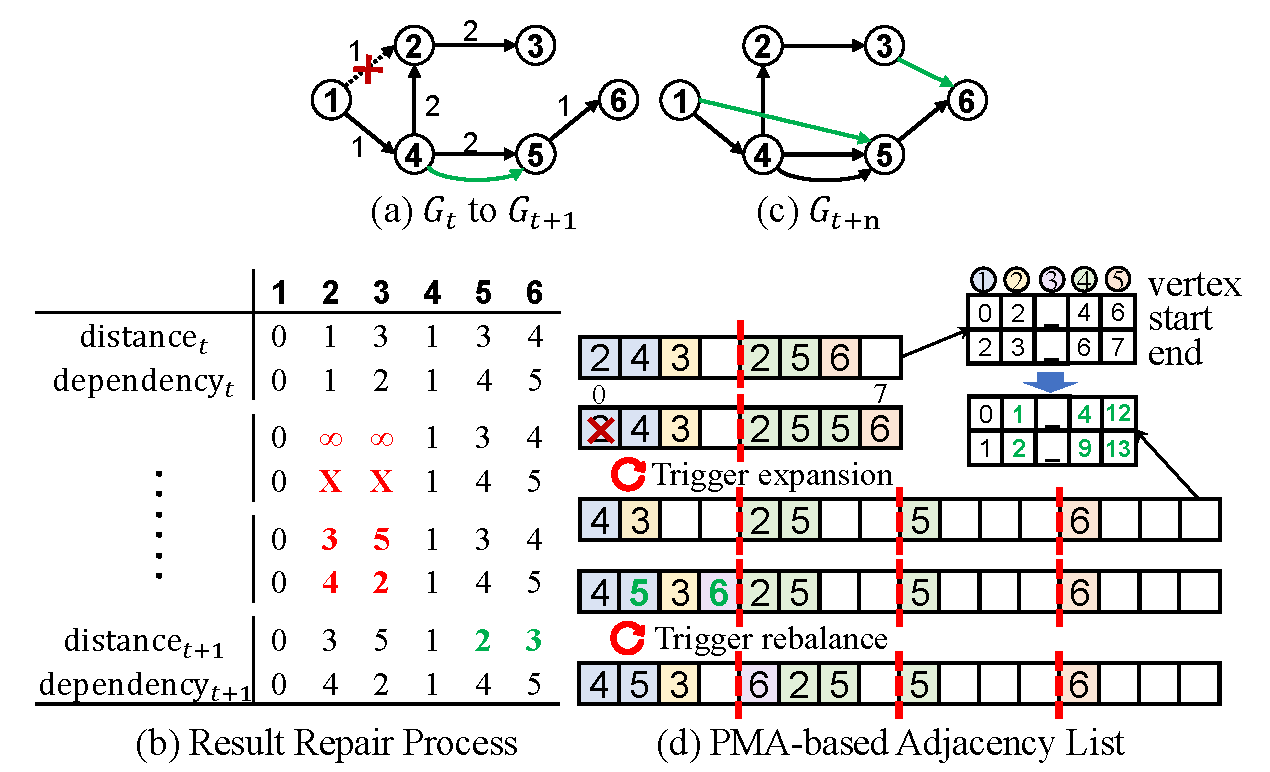
\includegraphics[width=\columnwidth]{figures/increment compute.pdf}
\caption{PMA-based adjacency maintenance and incremental result repair. (a)--(b) An edge update transforms $G_t$ into $G_{t+1}$ and propagates its effect to dependent vertices. (c) In the PMA, local shifts may change the indices of subsequent adjacency entries; insufficient local space triggers expansion, and density violations trigger rebalancing over a larger range. (d) The corresponding vertex results and dependencies are repaired to obtain the state for $G_{t+1}$.}
\label{fig:increment-compute}
\end{figure}

\subsection{Motivation}
\label{sec:motivation}

% 数据来源：paper/evaluation/raw/motivation_sssp_20261003/averages.csv（SSSP，TW/FS，100K，十批均值，counts/timing 各两次，Grapin=original）。
% Upd.=批内更新触及的源（去重）；Desc.=显式 H2D descriptor payload（MB=10^6 B；Grapin 约 16 B/顶点，CoIncGraph 约 24 B/源）；Init. WL=插入阶段初始 worklist 长度（CoIncGraph 即被插入边直接改善的终点数，与 seeds_prebatch 一致）。
% 未使用：Reloc.（Grapin 批边界净地址变化为 0）、|A|（Grapin 更小且两系统定义不同）、Rebuild 占比（5.3%/5.7%，说服力弱）、Seeds（与 CoIncGraph 的 Init. WL 重复）。
Out-of-memory streaming graph processing typically keeps the complete topology in host memory and places vertex results on the GPU, exploiting its high memory bandwidth and massive parallelism for computation, while adjacency is fetched from host memory over the PCIe bus on demand. Since PCIe bandwidth is far lower than device memory bandwidth, every adjacency transfer and every update to GPU-side graph views incurs substantial cost. Fortunately, streaming updates exhibit \textit{update locality}: in Twitter (TW) and Friendster (FS), a 100K-edge batch touches only 0.18\% and 0.15\% of the sources, respectively (Upd.\ in Table~\ref{tab:motivation}), so both costs should ideally scale with the changed region. However, we observe that existing designs lose this locality in both graph maintenance and incremental computation.

\begin{table}[t]
\centering
\caption{Per-batch statistics of SSSP (100K-edge batches, averaged over ten batches). Upd.: sources touched by the batch; Desc.: descriptor data transferred to the GPU; Init.\ WL: size of the initial insertion worklist.}
\label{tab:motivation}
\footnotesize
\setlength{\tabcolsep}{4pt}
\begin{tabular}{llrrr}
\hline
Graph & System & Upd. & Desc. (MB) & Init.\ WL \\
\hline
TW & Grapin~\cite{2025-Grapin} & 94,869 & 841.3 & 52,579,682 \\
 & CoIncGraph & 94,869 & 2.3 & 1,126 \\
\hline
FS & Grapin~\cite{2025-Grapin} & 99,188 & 1,049.7 & 65,608,366 \\
 & CoIncGraph & 99,188 & 2.4 & 1,684 \\
\hline
\end{tabular}
\end{table}

\textbf{Graph maintenance amplifies local updates.} Shared-array layouts, such as PMA or CSR, keep each source's adjacency contiguous for coalesced GPU access, but an insertion may shift, rebalance, or expand a range containing sources that receive no update. Since such relocations are decided inside the layout and cannot be derived from the update batch, publishing descriptors only for updated sources would risk leaving relocated sources pointing to stale locations; the descriptors of all $|V|$ vertices are therefore reloaded after every batch. As shown in Table~\ref{tab:motivation}, this transfers 841\,MB and 1,050\,MB of descriptors per batch in TW and FS, i.e., 16 bytes for every vertex, although fewer than 0.2\% of the sources are touched; publishing only the touched sources, as CoIncGraph does, reduces this volume to about 2\,MB. The GPU cache suffers similarly: modifying a cached source invalidates its cached adjacency, and the cache is evicted, compacted, and reloaded after every batch, even when the set of hot vertices barely changes. Consequently, maintenance cost scales with the graph rather than with the changed sources. This calls for a graph organization that confines relocation to updated sources, so that every CPU- and GPU-side graph view can be maintained at the granularity of changed sources.

\textbf{Incremental computation loses its affected region.} Restoring an invalidated vertex $v$ requires one of its remaining incoming edges, e.g., $(x,v)$, yet the predecessor $x$ is unaffected by the batch and thus inactive, and a GPU engine that traverses outgoing edges cannot locate it. Recovery is therefore merged into insertion processing, which reactivates all vertices and rebuilds worklists by scanning vertex states in every round~\cite{2025-Grapin}. As a result, the initial insertion worklist contains all 52.6M and 65.6M vertices in TW and FS, whereas only about 1.1K and 1.7K destinations are directly improved by inserted edges and need to start propagation, which is the initial worklist of CoIncGraph (Table~\ref{tab:motivation}). The missing incoming adjacency, however, is readily available on the CPU, which maintains the topology in host memory. If the CPU supplies the incoming edges of invalidated vertices, deletion repair can be completed within the affected region before insertions are applied, after which insertion propagation needs to start only from the improved vertices. This motivates decoupling deletion repair from insertion propagation through CPU--GPU cooperation and keeping worklists compact throughout. Sections~\ref{sec:graph-organization} and~\ref{sec:incremental-computation} present the designs that address these two observations.

\section{design of CoIncGraph}
\label{sec:design}

%  这一段还要重点修改一下，现在和最新的还没对应上

Figure~\ref{fig:1} presents an overview of CoIncGraph, a CPU--GPU cooperative system for incremental processing of streaming graphs that exceed GPU memory capacity. CoIncGraph integrates two components. First, a heterogeneous graph organization localizes adjacency changes and associated maintenance to changed sources. A unified change view coordinates updates to outgoing adjacency, the reverse index, and GPU views, avoiding redundant maintenance across these structures (Section~\ref{sec:graph-organization}). Second, a two-phase incremental execution pipeline performs deletion repair followed by insertion propagation. Compact worklists identify affected vertices: the CPU prepares incoming adjacency for GPU-based repair, while the GPU propagates improvements through outgoing edges (Section~\ref{sec:incremental-computation}). Together, these components confine data preparation and traversal to affected states and their dependencies, reducing redundant computation and CPU--GPU communication. In addition, CoIncGraph incorporates workload-specific optimizations to improve performance and broaden its applicability across diverse graph workloads (Section~\ref{sec:workload-cost}).

% We present a CPU--GPU cooperative system for out-of-memory streaming graph processing (Fig.~\ref{fig:1}). Section~\ref{sec:graph-organization}introduces a heterogeneous graph organization that confines adjacency changes and corresponding updates on the GPU and elsewhere to modified source vertices. A unified change view coordinates outgoing adjacency, the reverse index, and GPU views, reducing redundant maintenance across these structures. Building on this organization, Section~\ref{sec:incremental-computation} develops two-phase incremental computation: deletion repair followed by insertion propagation. Compact work lists identify affected vertices, guiding CPU preparation of incoming edges for GPU repair and GPU traversal from vertices whose results improve. This cooperation restricts data preparation and graph traversal to the affected computation and its dependencies, reducing redundant computation and CPU--GPU communication.

\begin{figure}[t]
\centering
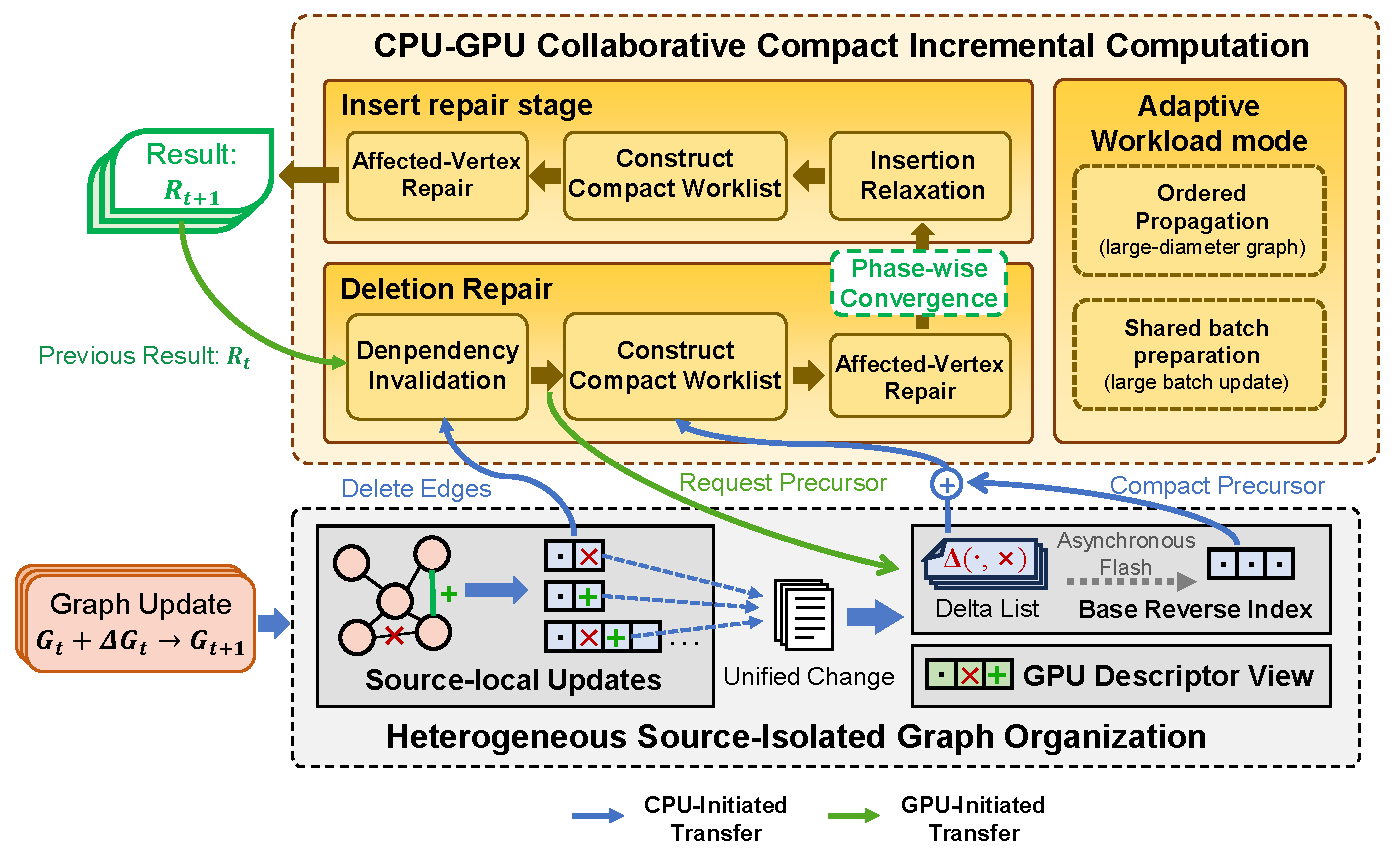
\includegraphics[width=\columnwidth]{figures/Overview.pdf}
\caption{The Overview of CoIncGraph System.}
\label{fig:1}
\end{figure}

\subsection{Heterogeneous Source-Isolated Graph Organization}
\label{sec:graph-organization}

Section~\ref{sec:motivation} shows that shared-array layouts transform a local update into the relocation of unrelated sources, resulting in extensive descriptor modifications and per-batch cache reorganization. The key idea of our graph organization is to \textit{make the source vertex of an update edge the unit of storage, change description, and GPU publication}, so that maintenance cost follows the set of changed sources rather than the graph size. It consists of three mechanisms. \textit{Source-isolated adjacency blocks} allocate each source's adjacency independently, so that an update never relocates other sources. A \textit{unified change view} resolves each batch once into effective edge changes and changed sources that drive all graph views. \textit{Selective view maintenance} uses this view to update the reverse index, publish GPU descriptors, and repair cached adjacency only for changed sources.

% Topological locality offers an opportunity to limit adjacency movement and GPU index maintenance to the sources whose outgoing adjacency changes in a batch. However, insertion operations in the PMA structure may trigger rebalancing, causing the adjacency list to be migrated to a locality other than that of the source vertex, thereby increasing the volume of data movement and the overhead of index maintenance at other locations. We organize maintenance around independently allocated source blocks. Section 4.1 explains how this layout prevents updates from relocating unrelated lists. Section 4.2 coordinates updates to outgoing and incoming adjacency through a common batch plan. Section 4.3 uses the resulting changed-source set to update only the required GPU adjacency indices while preserving consistent graph access.

\subsubsection{Source-Isolated Adjacency Blocks}
\label{sec:source-layout}
Relocation in shared arrays arises because the adjacency of different sources shares one address space, so the space required by one source is obtained by moving its neighbors. We therefore make the source the unit of allocation. The graph resides in pinned host memory mapped into the GPU address space, and each source stores its neighbors in an independently allocated, contiguous block with spare capacity, which the GPU locates through the source's adjacency descriptor. An insertion appends neighbors in place when the block has sufficient capacity; otherwise, the CPU allocates a larger block, copies only this source's adjacency, and appends the new neighbors. A deletion removes the requested edges that exist and compacts the remaining neighbors within the same block.

% 这块的图后面看看能不能画个这个数据结构对应的图（不行就需要把这块的图给删除）
This organizational approach ensures that the adjacency relationships of a source change only when the source itself updates. The descriptors and cached adjacency of all other sources therefore remain valid, which makes it safe to publish GPU-side changes only for changed sources. As illustrated in Fig.~\ref{fig:view}, expanding $w$'s block leaves all other blocks and descriptors untouched, whereas the same insertion in a PMA shifts and rebalances unrelated  elements. Since each block keeps its neighbors contiguous, the coalesced zero-copy access of compact layouts is preserved.

% The graph resides in host memory. For each source, the GPU maintains an adjacency descriptor, an index record that identifies where its neighbor list is stored and how many neighbors it contains. Although graph updates are local, modifying a few vertices can relocate the adjacency lists of many unchanged vertices, requiring corresponding updates to their GPU indices and thereby amplifying the data update overhead. To confine this maintenance to updated sources, we allocate and grow each source's adjacency independently.

% Each source $u$ stores its neighbors in an independently allocated, contiguous block of mapped host memory, with spare capacity for insertions. For insertions, the CPU appends new neighbors to $u$'s existing block if its capacity is sufficient. Otherwise, it allocates a larger block, copies $u$'s existing adjacency into it, and appends the new neighbors. Expansion uses a separately allocated block, leaving the locations of other adjacency lists unchanged. Figure~\ref{fig:2}(a) contrasts the proposed design with a shared PMA. In the PMA, even local data shifts before rebalancing may change the indices of other source vertices whose adjacency lists remain unchanged. In contrast, expanding the private memory block of $w$ in our design does not affect the memory blocks of other source vertices or invalidate their descriptors. For deletions, the CPU removes the specified edges that exist in the graph and compacts the remaining neighbors within the existing block. This preserves the contiguous neighbor access of the original layout while restricting relocation to the updated source.

% Independent block allocation eliminates cross-source redistribution, preserving the adjacency locations and descriptors of unchanged sources. This confines relocation costs to updated lists and enables sparse GPU publication (Section~4.3). Expansion and deletion may still copy or scan an entire updated list, while spare capacity and delayed block reclamation incur memory overhead.

\subsubsection{Unified Change View}
\label{sec:change-view}
% A topology view is a representation of graph in a particular data structure or on a particular device, organized for the access it supports. Our system maintains three such views. Outgoing adjacency stores each source's neighbors in host memory for traversing its outgoing edges. The reverse index stores the sources of incoming edges for each destination, allowing deletion recovery to find the remaining predecessors that may restore its distance. GPU adjacency descriptors store each source's neighbor-list location and degree, allowing GPU computation to locate and read its outgoing neighbors. Each topology update must be reflected in all three views. We coordinate their maintenance through a unified change view, consisting of effective edge-change records and changed-source lists produced during outgoing-adjacency preparation for each update phase.

% The CPU groups update requests by source so that each adjacency list is scanned and modified at most once per phase. For each source, it collects all deletion requests and records how many existing edges to each destination should be removed. It then removes these edges together by compacting the neighbor list once, avoiding repeated movement of the same entries when edges are deleted one at a time. It also determines the capacity required for the source's insertions as a group. If the current block is too small, the CPU allocates a larger block and copies the existing neighbors once before appending the new edges. Thus, grouping reduces repeated movement within an updated adjacency list, complementing the isolation of movement across sources in Section 4.1. Independent source blocks allow the compaction and append operations for different sources to proceed in parallel.

% Grouping updates by source also provides the information needed to maintain the other topology views. During preparation, the CPU records each source--destination pair and the number of edges actually removed or added, together with the sources whose adjacency changes. Unsuccessful deletion requests produce no change. The reverse index uses the edge records to update incoming adjacency, while GPU descriptor and cache updates use the source lists to locate the outgoing lists that have changed. These structures therefore reuse the results of adjacency preparation instead of independently determining the effects of the same requests.

% For example, suppose source $u$ has neighbors $[a,a,b]$ and receives three requests to delete $(u,a)$ and one to insert $(u,c)$. Only two copies of $(u,a)$ exist, so deletion compacts the list to $[b]$ and produces the record $(u,a,-2)$. The reverse index uses this record to remove the two incoming edges from $u$ at $a$. Insertion later produces $[b,c]$ and the record $(u,c,+1)$, which adds an incoming edge from $u$ at $c$. Both stages identify $u$ as changed. The system then updates its GPU descriptor and, if present, its cached adjacency, as illustrated in Fig.~\ref{fig:2}(b). The third deletion request causes no additional index update.

Source isolation bounds where adjacency moves, but each batch must still be reflected in several graph views: the host outgoing adjacency for traversal, a host reverse index that provides incoming adjacency for deletion repair, and the GPU descriptors and cached adjacency used by computation. Deriving the changes of each view independently from the update requests would repeat the same validation, and a deletion request that matches no existing edge could even make the views inconsistent. We instead resolve the requests once against the outgoing adjacency and record the outcome in a \textit{unified change view}, which consists of effective edge-change records and changed-source lists generated in each update phase. The reverse index consumes the edge-change records, while GPU descriptor and cache maintenance consume the changed-source lists.

The CPU groups requests by source and determines their effects against the graph state at the start of each phase. The deletion operation removes existing edges by compacting the affected list. The insertion operation first determines whether the current block requires expansion before performing the addition. Grouping reduces repeated movement within lists, complementing source isolation across lists and allowing outgoing-adjacency updates for different sources to proceed in parallel. Preparation records the number of edges actually removed or added for each source--destination pair and identifies changed sources. Unsuccessful deletions therefore produce no change records.

%\textbf{Large-batch preparation.} For small batches, each maintenance stage (block allocation, adjacency mutation, and reverse-index preparation) builds its own compact copy of the per-source plan and effective records, which costs little and keeps accesses sequential. With millions of updates per batch, however, these copies grow with the batch, and repeated preparation, copying, and sorting become a major CPU cost. CoIncGraph therefore switches to a large-batch mode when a batch contains at least one million updates. In this mode, the CPU keeps a single per-source plan indexed by changed sources, which is shared by change-record generation, block allocation, adjacency mutation, and block reclamation; the effective records are moved, rather than copied, into reverse-index preparation; and since both phases emit changed sources in source order, the two lists are merged linearly for publication instead of being sorted again. This mode changes only how preparation results are stored and shared, not the effective changes they describe.

For example, suppose $u$ has neighbors $[a,a,b]$ and receives three deletion requests for $(u,a)$. Deletion removes the two existing copies, produces $[b]$, and emits $(u,a,-2)$ for reverse-index maintenance, while the unmatched third deletion request triggers no maintenance operation in any view. Then, the edges $(w,c)$ and $(w,d)$ are inserted, triggering an expansion and emitting $(w,c,+1)$ and $(w,b,+1)$. Consequently, vertex $v$ remains unaffected by any operations involving other vertices throughout this entire phase, as illustrated in Fig.~\ref{fig:view}.

For large batches with millions of updates, however, building a separate copy of these plans and records for every maintenance stage makes repeated preparation, copying, and sorting a dominant CPU cost. We therefore adopt \textbf{shared batch preparation}, in which a single per-source plan is shared by change-record generation, block allocation, and adjacency mutation. The effective records are handed over to reverse-index maintenance without copying. Since both phases emit changed sources in source order, the two lists are merged linearly for publication rather than sorted again. This optimization changes only how preparation results are stored and reused, not the effective changes they describe.


\begin{figure}[t]
\centering
\includegraphics[width=\columnwidth]{figures/view.pdf}
\caption{Source-Isolated Adjacency Blocks and Unified Change View.}
\label{fig:view}
\end{figure}


\subsubsection{Selective View Maintenance}
\label{sec:view-maintenance}


% \textbf{Reverse index maintenance.} Maintaining incoming adjacency directly from the input requests would cause other views to repeat checks already performed when processing outgoing adjacency. To avoid this work, the reverse index consumes the actual edge changes, groups them by destination, and combines changes for the same source--destination pair. Each destination stores a sorted base list of incoming sources and a separate list of delta records. A delta record contains a source vertex and the net number of edges added or removed relative to the base list: a positive value indicates additions, and a negative value indicates deletions. New changes are merged into these records, and records with a zero net change are removed. This avoids checking deletion requests again and modifying the base lists for every update. This CPU-maintained structure enables subsequent GPU operations to directly query the current incoming neighbors of affected target nodes, without the need to reconstruct incoming adjacency relationships based on all outgoing lists and update information.

% To retrieve the current incoming neighbors of a destination, the index counts the occurrences of each source in the base list and adds the value in its delta record, if one exists. A source is returned if the resulting count is positive. For example, a base list $[u,u,w]$ and delta records $[(u,-2),(v,+1)]$ yield incoming sources $[v,w]$: both edges from $u$ have been removed, the edge from $w$ remains, and an edge from $v$ has been added. The base list remains unchanged during updates, while the delta records provide the current incoming view at query time.


% \textbf{GPU descriptor and cache maintenance.} Reloading all GPU descriptors after a local update would transfer indices for many vertices whose adjacency remains unchanged. Source isolation makes these transfers unnecessary, while the source lists produced during adjacency maintenance identify the descriptors that need updating. Let $S^-$ and $S^+$ denote the sources changed during deletion and insertion. The system forms $S=S^-\cup S^+$ so that each source is included once, even if it changes in both stages. Sources with only unsuccessful deletion requests are excluded. After insertion, the CPU transfers one record per source in $S$, containing its final adjacency location, degree, and version, and the GPU writes these records into the corresponding descriptor entries. Since these records are generated during topology maintenance on the CPU, the descriptor updates on the GPU correspond to the source vertices where changes actually occurred, rather than the volume of data in the original updates. Sources outside $S$ retain valid descriptors because their adjacency has not moved or changed.

% Each descriptor update occupies 24 bytes, giving a transfer volume of $24|S|$ bytes per batch. Descriptor traffic therefore scales with the number of changed sources rather than the total vertex count. Incoming-neighbor transfers, cached-list copies, and accesses to host adjacency incur separate costs.

% The source list also limits the repair of cached adjacency. If a changed source has a valid GPU cache entry, the system copies its current neighbor list into the existing space when it fits. Otherwise, it attempts to place the list in unused space at the end of the cache and updates its cache index. If there is insufficient space, it invalidates the cached copy, allowing computation to read the current host adjacency. Each repair copies the changed source's entire neighbor list; cached lists of other sources are left in place during this step.

% To prevent GPU computation from reading stale indices or cached neighbors, descriptor and cache updates run in one CUDA stream, and subsequent computation waits for them to finish. Replaced host blocks are reused only after earlier GPU readers have completed, preventing access to reclaimed adjacency storage.

% Local repair can also avoid subsequent cache reorganization. After computation, the existing hotness-based policy selects the vertices to cache. If all selected vertices have valid cached adjacency and their number matches the previously published cache set, the system skips eviction, compaction, and loading. Otherwise, it performs the normal cache replacement procedure. This prevents a local topology change from unnecessarily triggering the full cache maintenance sequence, while still allowing replacement when the selected vertices change or local repair cannot retain a valid copy.

% Together, source isolation, shared change records, and selective GPU updates confine adjacency relocation and cache repair to changed sources, while avoiding repeated processing of the same updates across topology indices. They reduce both data movement and the additional index maintenance.

We coordinate reverse-index, GPU descriptor, and cache maintenance through the unified change view, avoiding repeated update validation and unnecessary data movement. The reverse index groups effective edge changes by destination and aggregates them by source--destination pair. Each destination maintains a sorted base list of predecessors and delta records tracking net changes in edge multiplicity. Updates modify only the deltas, removing zero-valued records rather than rewriting the base list. Queries obtain current predecessors by adding each source's delta to its base multiplicity and retaining positive counts. For example, base list $[u,u,w]$ with deltas $[(u,-2),(v,+1)]$ yields predecessors $[v,w]$. This representation supports deletion repair without rechecking input requests or reconstructing incoming adjacency from outgoing lists.

Source isolation further enables selective maintenance of the GPU views, i.e., descriptor publication and cache repair only for changed sources. Let $S^-$ and $S^+$ denote sources changed during deletion and insertion. After insertion, the CPU publishes one descriptor record per source in $S=S^-\cup S^+$, containing its final adjacency location, degree, and version. Sources outside $S$ retain valid descriptors, and unsuccessful deletions generate no publication records. With 24-byte records, descriptor traffic is $24|S|$ bytes per batch rather than proportional to the total vertex count. Cache repair likewise targets only changed sources: each cached list is refreshed in place if it fits, relocated to unused cache-tail space otherwise, or invalidated if space is insufficient. Each repair copies the source's entire current adjacency, while other cached lists remain in place. Transfers of incoming adjacency and accesses to host adjacency incur separate costs.

To preserve consistent access, descriptor and cache updates execute in one CUDA stream, subsequent computation waits for completion, and replaced host blocks are reclaimed only after earlier GPU readers finish. After computation, the hotness-based policy selects the next cache set. If it matches the previously published set and all selected entries remain valid, the system skips eviction, compaction, and loading; otherwise, it performs normal replacement. Coordinating selective publication with local cache repair thus avoids full descriptor reloads and unnecessary cache reorganization while preserving adaptation to changing workloads.

\subsection{Cooperative Compact Incremental Computation}
\label{sec:incremental-computation}
As discussed in Section~\ref{sec:motivation}, the lack of GPU-side predecessor access defers deletion repair to insertion processing, requiring global vertex reactivation and worklist reconstruction. Our key idea is to complete deletion repair before applying insertions, using incoming adjacency supplied by the CPU. Once results are correct for the post-deletion graph, insertion propagation can start solely from destinations improved by inserted edges. Without this separation, such selective propagation may miss alternative paths through inactive predecessors, such as $(x,v)$ in Section~\ref{sec:motivation}. We therefore introduce two mechanisms: \textit{Cooperative Deletion Repair} combines GPU-side identification of affected vertices with CPU-side incoming adjacency preparation to restrict repair to the affected region; \textit{Compact Insertion Propagation} starts from improved destinations and directly constructs compact worklists from successful updates.
% As discussed in Section~\ref{sec:motivation}, the GPU cannot locate the predecessors of invalidated vertices, so their recovery is merged into insertion processing, which reactivates all vertices and rebuilds worklists over the entire graph. The key idea of our incremental computation is to complete deletion repair on the graph after deletion before applying any insertion, using the incoming edges of affected vertices supplied by the CPU. Once deletion repair converges, every result is correct for the graph after deletion; any further change can then originate only from destinations improved by inserted edges, so insertion propagation needs to start only from these destinations. Without this decoupling, starting from inserted edges alone would miss alternative paths through inactive predecessors, such as $(x,v)$ in Section~\ref{sec:motivation}. Building on this property, we design two mechanisms. \textit{cooperative deletion repair} lets the GPU identify the affected vertices, while the CPU prepares their incoming edges from the host-resident data that is not available on the GPU, confining repair to the affected region. \textit{cooperative insertion propagation} seeds propagation only with improved destinations and builds compact worklists directly from successful updates.

% Updates to the streaming graph are localized, yet work list construction and incremental maintenance can still process unaffected vertices. We reduce this overhead through CPU--GPU cooperative incremental computation. Section 5.1 uses affected vertices identified by the GPU to retrieve only the predecessor lists needed for deletion repair from the CPU-maintained reverse index. Section 5.2 publishes changed topology and propagates insertion effects only from vertices whose results improve. Section 5.3 reduces repeated propagation and large-batch preparation costs.

\subsubsection{Cooperative Deletion Repair}
\label{sec:deletion-repair}
We describe the process using SSSP with positive edge weights (BFS uses unit weights). A vertex result is its current distance estimate, denoted by $d(v)$, and a better result corresponds to a smaller estimate in this example. For a batch of effective deletions $D_t$ and insertions $I_t$, let $G_t=(V,E_t)$ be the previous graph. The graph after deletion is $G_{t+1}^{-E}=(V,E_t\setminus D_t)$, and the final graph is $G_{t+1}^{+E}=(V,(E_t\setminus D_t)\cup I_t)$. Algorithm~\ref{alg:process-batch} summarizes the CPU--GPU cooperative workflow of a batch, which starts by grouping the requests by source (Line~\ref{ln:group}). The subsequent steps are as follows.

\begin{algorithm}[t]
\caption{CPU--GPU cooperative processing of an update batch.}
\label{alg:process-batch}
\small
\begin{algorithmic}[1]
\Require Graph $G_t$, vertex results, deletions $D_t$, insertions $I_t$
\Ensure Graph $G_{t+1}^{+E}$ and its converged vertex results
\State \textbf{CPU:} $P \gets \Call{GroupBySource}{D_t,I_t}$ \label{ln:group}
\Statex \textit{Step 1: Dependency invalidation (GPU)}
\State $A \gets \Call{InvalidateAndAppend}{G_t,D_t}$ \Comment{Compact worklist} \label{ln:inv}
\State \Call{ResetResults}{$A$}; transfer $A$ to the CPU \label{ln:reset}
\Statex \textit{Step 2: Incoming-adjacency preparation (CPU)}
\State $S^- \gets \Call{ApplyDeletionsAndUpdateReverse}{P}$ \label{ln:applydel}
\State $I(A) \gets \Call{MaterializeIncoming}{A}$; transfer $I(A)$ to the GPU \label{ln:incoming}
\Statex \textit{Step 3: Deletion repair (GPU)}
\Repeat \label{ln:repair-begin}
    \ForAll{$v \in A$ \textbf{in parallel}}
        \State \Call{PullRelax}{$v, I(A)$} \Comment{Eq.~(\ref{eq:pull})}
    \EndFor
\Until{no result in $A$ changes} \Comment{Checked by the CPU} \label{ln:repair-end}
\Statex \textit{Step 4: Topology publication (CPU--GPU)}
\State \textbf{CPU:} $S^+ \gets \Call{ApplyInsertionsAndUpdateReverse}{P}$ \label{ln:applyins}
\State \Call{PublishAndRepairCache}{$S^- \cup S^+$}; wait for completion \label{ln:publish}
\Statex \textit{Step 5: Initial worklist construction (GPU)}
\State $L \gets \Call{RelaxInsertionsAndAppend}{I_t}$ \label{ln:seed}
\Statex \textit{Step 6: Insertion propagation (one cooperative GPU kernel)}
\While{$L \neq \emptyset$} \label{ln:prop-begin}
    \State $L_{\mathrm{next}} \gets \emptyset$
    \ForAll{$u \in L$ \textbf{in parallel}}
        \If{\Call{CommitLatestImprovement}{$u$}} \label{ln:commit}
            \ForAll{outgoing edges $(u,v)$ in $G_{t+1}^{+E}$}
                \If{\Call{AtomicRelax}{$u,v$} succeeds} \label{ln:relax}
                    \State \Call{AppendOnce}{$v,L_{\mathrm{next}}$} \label{ln:append}
                \EndIf
            \EndFor
        \EndIf
    \EndFor
    \State \Call{GridSynchronize}{}; \Call{Swap}{$L,L_{\mathrm{next}}$} \label{ln:prop-end}
\EndWhile
\end{algorithmic}
\end{algorithm}

\textbf{Step 1: Dependency invalidation (Lines~\ref{ln:inv}--\ref{ln:reset}).} Following dependency-memoization, a deletion invalidates the results of all vertices whose dependencies pass through the deleted edge, and these vertices must be reset before repair. Collecting them by scanning vertex marks across all graph partitions would examine the entire graph in every round, although the invalidated region is typically small. We instead build a compact worklist directly as vertices are marked.

The GPU initializes an empty worklist $L_{\mathrm{del}}$ and examines the deleted edges in parallel. For each deleted edge $(u,v)$, it marks $v$ if the current result of $v$ depends on that edge, and only the thread that first marks $v$ atomically reserves a slot and appends $v$ to $L_{\mathrm{del}}$. Each subsequent round scans, in $G_t$, the outgoing edges of the vertices appended in the preceding round and appends newly marked dependents in the same way, yielding a breadth-first traversal of dependencies. When a round appends no vertex, $L_{\mathrm{del}}$ holds exactly the affected vertices, denoted by $A$: each appears once in consecutive slots, and unaffected vertices occupy no slot. The GPU resets the stored and tentative results of $A$ to $\infty$ and transfers their IDs to the CPU. $A$ thus serves as the interface between the two processors: it determines exactly which incoming adjacency the CPU prepares for repair.

\textbf{Step 2: Preparing incoming adjacency (Lines~\ref{ln:applydel}--\ref{ln:incoming}).} An affected vertex may regain its result through an unaffected predecessor whose result has not changed. For example, after deleting $(u,v)$, the remaining edge $(x,v)$ may restore $v$ even though $x$ is inactive. Repair therefore requires the remaining incoming adjacency of the vertices in $A$:

\begin{equation}
I(A)=\{(u,v)\in E(G_{t+1}^{-E})\mid v\in A\}.
%\tag{5.1}
\end{equation}

The GPU supplies only the IDs in $A$, and the CPU obtains their predecessors from the reverse index (Section~\ref{sec:view-maintenance}), which already reflects the effective deletions of the batch. For each $v\in A$, the CPU merges the base list and the delta records of $v$ in source order and retains sources with positive multiplicity. Predecessor discovery is thus confined to the reverse-index of $A$, without scanning the outgoing adjacency of any source.

When $A$ is large, the CPU splits it into fixed-size tiles of consecutive destinations and processes them with a persistent pool of worker threads. Workers claim tiles dynamically through an atomic counter, one tile at a time, so that tiles containing high in-degree destinations do not stall the other workers. Each worker merges the incoming adjacency of its tile into a private buffer and records the length $\ell_i$ of each list. After all tiles are merged, an exclusive prefix sum $o_i=\sum_{k<i}\ell_k$ gives each destination $a_i$ a disjoint output range $[o_i,o_{i+1})$, so workers copy their buffers into the final array in parallel without atomic appends or locks, while preserving the order of $A$. Each destination's records are therefore merged only once.

The result stores the incoming adjacency of each destination contiguously, with offsets delimiting the lists in the order of $A$. The CPU transfers these offsets and source IDs to the GPU, while vertex results remain on the GPU. With $M_A$ incoming-adjacency entries, this representation occupies $O(|A|+M_A)$ space, and its construction work is proportional to $|A|$ plus the base and delta records examined for these destinations. \textit{Consequently, the data prepared by the CPU and transferred for repair is determined by the affected region rather than by the graph size.}

\textbf{Step 3: Repairing vertex results (Lines~\ref{ln:repair-begin}--\ref{ln:repair-end}).} Using the prepared incoming edges, the GPU repeatedly improves the result of each $v\in A$ with candidates from its predecessors. For SSSP, this pull-based update is:

\begin{equation}
d(v)\leftarrow\min\left\{d(v),
\min_{(u,v)\in I(A)}[d(u)+w(u,v)]\right\}.
%\tag{5.2}
\label{eq:pull}
\end{equation}

A warp cooperatively scans the incoming adjacency of each affected vertex, and improved results of affected vertices serve as candidates for their affected successors in later rounds. Vertices without any remaining path keep the result $\infty$.

After step 3, all results are correct for $G_{t+1}^{-E}$, while repair has examined only $A$ and $I(A)$. This stable state is the precondition of the compact insertion propagation in Section~\ref{sec:insertion-propagation}: since no invalidated result remains, the inserted edges are the only source of further changes.

\subsubsection{Compact Insertion Propagation}
\label{sec:insertion-propagation}

\textbf{Step 4: Publishing the updated graph (Lines~\ref{ln:applyins}--\ref{ln:publish}).} After deletion repair, the CPU applies the insertions, updates the reverse index, and forms the changed-source set $S=S^-\cup S^+$. It then publishes the final descriptors of $S$ and repairs their cached adjacency (Section~\ref{sec:view-maintenance}). Once publication completes, the GPU traverses the final graph without a full descriptor reload.

\textbf{Step 5: Building the initial worklist (Line~\ref{ln:seed}).} Since deletion repair has already restored all results, only destinations improved by inserted edges can initiate further changes. After publication, GPU threads relax the inserted edges in parallel with atomic minimum updates, and each destination whose tentative result improves is appended at most once to the initial worklist, using the same append-on-change construction as step 1. The initial worklist therefore contains at most $|I_t|$ vertices instead of all $|V|$ vertices, and the subsequent adjacency traversal starts only from vertices whose results have actually improved.

\textbf{Step 6: Propagating result improvements (Lines~\ref{ln:prop-begin}--\ref{ln:prop-end}).} For each vertex in the current worklist, a GPU thread block checks whether its latest tentative result is better than its stored result. If so, it commits the improvement (Line~\ref{ln:commit}) and reads the vertex's contiguous outgoing adjacency through its published descriptor, either from the hot-subgraph cache or from host memory via zero-copy access. Whenever an edge improves its destination's tentative result, the destination is appended to the next worklist (Lines~\ref{ln:relax}--\ref{ln:append}). An atomic minimum preserves the best concurrent update, and a per-vertex tag containing the batch and round admits each destination at most once per round, while a later improvement may admit it again in a subsequent round. Successful updates thus construct the next worklist directly, and no round scans unrelated vertices to rebuild worklists.

With compact worklists, later rounds often contain only a few active vertices, so per-round host coordination, including kernel launches, worklist exchange, and convergence checks, can outweigh the useful work. We therefore execute insertion propagation within a single cooperative GPU kernel. The GPU maintains the current and next worklists, uses grid-wide barriers to complete pending writes before exchanging them (Line~\ref{ln:prop-end}), and terminates when the next worklist is empty; the CPU only waits for the kernel to finish. This removes host orchestration and repeated kernel launches between insertion rounds.

Let $X_k$ be the vertices whose results improve and whose outgoing edges are examined in round $k$. The edge work is

\begin{equation}
W_{\mathrm{expand}}=
\sum_k\sum_{u\in X_k}\deg^+_{G_{t+1}^{+E}}(u).
%\tag{5.3}
\end{equation}

Vertices without improvements never read their adjacency, which reduces both edge processing and requests to host memory. Repeated improvements of the same vertex may still cause repeated reads, which ordered propagation reduces (Section~\ref{sec:ordered-propagation}).


\subsubsection{Ordered Propagation}
\label{sec:ordered-propagation}
\label{sec:workload-cost}
Compact worklists exclude vertices whose results do not change, but they cannot prevent the same vertex from being activated repeatedly by successively better results. In large-diameter graphs such as road networks, updates propagate over many rounds, and propagating every intermediate improvement immediately triggers repeated scans of downstream adjacency that are later superseded. Inspired by ~\cite{2014-bucket}, we impose a priority order on pending vertices. For instance, in algorithms where a smaller value is preferable, ordered propagation prioritizes vertices with smaller tentative values, so that deferred vertices can receive further improvements before scanning their outgoing edges. The GPU assigns each pending vertex with tentative value $r$ to bucket $\lfloor r/\Delta\rfloor$, where $\Delta>0$ is the bucket width, processes the smallest nonempty bucket, and retains the other vertices for later rounds. This ordering changes only the order in which pending vertices are served in deletion repair (Lines~\ref{ln:repair-begin}--\ref{ln:repair-end}) and insertion propagation (Lines~\ref{ln:prop-begin}--\ref{ln:prop-end}). We enable this ordering for large-diameter graphs. It reduces redundant edge scans and host-memory accesses at the cost of more rounds, and is therefore not used for low-diameter graphs, where propagation converges in a few rounds.

\section{Evaluation}
\subsection{Experiment Setup}
% 实验环境
\subsubsection{Experimental Environment} We implement our system in C++ and CUDA and evaluate it on a server with two Intel Xeon Gold 5218R processors (80 physical cores in total) and an NVIDIA V100 GPU. Each CPU has a base frequency of 2.10 GHz. The V100 has 80 streaming multiprocessors (5,120 CUDA cores) and 16 GB of global memory. The GPU connects to the host via PCIe 3.0 $\times$16, with a theoretical peak bandwidth of approximately 16 GB/s per direction. We compile the code with NVIDIA NVCC 13.0 and GCC 13.3.0 using the \texttt{-O3} optimization flag.  % 这块软硬件环境，后面需要和绍炎核对一下。
% 数据集
\subsubsection{Datasets} % 数据集都是从哪下载的，需要引用一下地址
We evaluate CoIncGraph on six real-world graphs whose statistics are summarized in Table~\ref{tab:datasets}. OK~\cite{OKFS}, WK~\cite{WK}, TW~\cite{TW}, and FS~\cite{OKFS} are social networks with power-law degree distributions, whereas EU and USA are road networks with large diameters. Following Grapin and GraphBolt~\cite{2025-Grapin,2019-GraphBolt}, we uniformly sample edges without replacement and assign half to insertions and half to deletions. We remove the insertion edges from the original graph to form the initial graph $G_0$, then randomly interleave the updates and partition them into ten equal-sized batches, each containing equal numbers of insertions and deletions.
% Table~\ref{tab:datasets} presents the six real-world graph datasets used in our study. OK, WK, TW, and FS are social networks—characterized by power-law distributions—while EU and USA are road networks, which possess larger diameters. Our streaming workload construction follows the approach used in [Grapin, Graphbolt]. First, we perform uniform sampling of edges from the original graph without replacement; half of the sampled edges are designated for insertion and the other half for deletion. The edges designated for insertion are excluded from the original graph to form the initial graph, $G_0$. The resulting update operations are randomly interleaved and partitioned into ten consecutive batches, with each batch containing an equal number of insertion and deletion operations. This method effectively preserves the edge distribution characteristics of the datasets.

% 这块后面可以看看要不要加直径（Diameter） 对应平均度，针对有向和无向图有区别
\begin{table}[t]
\centering
\caption{Dataset used for the experiment.}
\label{tab:datasets}
\footnotesize 
\setlength{\tabcolsep}{2pt}
\begin{tabular}{ccccc}
\hline
Graph & Vertices & Edges & $\overline{Degree}$ & Diameter \\
\hline
Orkut (OK)\ \cite{OKFS} & 3,072,441 & 117,185,083 & 76.28 & 9 \\
Wikipedia (WK)\ \cite{WK} & 13,593,032 & 437,217,424 & 32.16 & 10  \\
Twitter-2009 (TW)\ \cite{TW} & 52,579,682 & 1,963,263,821 & 37.34 & 18 \\
Friendster (FS)\ \cite{OKFS} & 65,608,366 & 1,806,067,135 & 55.06  & 32 \\
Europe OSM (EU)\ \cite{eu} & 50,912,018 & 54,054,660 & 2.12  & 30,102 \\
USA Road (USA)\ \cite{usa} & 23,947,347 & 28,854,312 & 2.41 & 8,440 \\
\hline
\end{tabular}
\end{table}

% 对比基线
\subsubsection{Baselines} We compare CoIncGraph with three state-of-the-art systems: Ingress, SHGraph, and Grapin. SHGraph~\cite{2020-SHGraph}, Gunrock's dynamic graph module, uses per-vertex Slab Hash tables to support parallel graph updates and queries in GPU memory. Ingress~\cite{2021-Ingress} performs CPU-based incremental graph processing and automatically selects a memoization policy (memoization-free, memoization-path, memoization-vertex, or memoization-edge) according to the algorithm properties, so that only the memoized states required by the algorithm are maintained and revised. Grapin~\cite{2025-Grapin} supports CPU--GPU cooperative out-of-memory (OOM) streaming graph processing by maintaining graph topology in host memory and executing incremental computation on the GPU. It combines GPU hot-subgraph caching with optimized zero-copy access to reduce CPU--GPU data movement.
% 后面可以考虑，看要不要评估方法的简单说明，大概一段
\subsubsection{Methodology} We evaluate all systems on [graph algorithms] using identical initial graphs and update sequences. We measure end-to-end processing time and update throughput (processed update edges per second), including graph updates, incremental computation, and CPU--GPU transfers where applicable, but excluding initial graph loading and preprocessing. Speedup is the ratio of baseline processing time to that of CoIncGraph. We report the arithmetic mean of five independent runs, each starting from the same initial graph. We also examine sensitivity to [batch size and other parameters] and quantify individual optimizations through ablation studies.
% \subsubsection{Baselines} 
% We compare our system with three state-of-the-art systems, covering GPU-based in-memory dynamic graph processing, CPU-based incremental processing, and CPU-GPU collaborative OOM streaming graph processing.

% \noindent\textbf{Gunrock dynamic (SHGraph).}
% Gunrock's dynamic graph module~\cite{2020-SHGraph}, referred to as SHGraph, represents GPU-resident dynamic graph processing. It uses per-vertex Slab Hash tables to support efficient parallel graph updates and queries within GPU memory.

% \noindent\textbf{GraphBolt.}
% GraphBolt~\cite{2019-GraphBolt} represents CPU-based incremental streaming graph processing. It tracks dependencies among intermediate values across iterations to propagate graph updates while reusing unaffected computation and preserving bulk synchronous parallel (BSP) semantics.

% \noindent\textbf{Grapin.}
% Grapin~\cite{2025-Grapin} represents CPU--GPU cooperative out-of-memory streaming graph processing, maintaining graph topology in host memory and performing incremental computation on the GPU. It combines GPU hot-subgraph caching with optimized zero-copy access to reduce host-to-device data transfers.

\subsection{Overall Performance}
\label{sec:overall}
% 这部分撰写整体的实验性能
% 数据来源：paper/evaluation/data/performmance.csv（每个配置2次重复取均值，10个batch累计时间）。
% 加速比统计口径：几何平均（geometric mean）。
% Ingress计时窗口为reset+compute，不含其全图拓扑重建（比current/Grapin窗口更窄，对Ingress有利，因此加速比偏保守）；TW/FS的Ingress为单次运行结果，需补齐第二次。
% EU、USA两个路网图尚未纳入本表，后续补齐后需同步更新Table与文中的统计数字。

\begin{table*}[t]
\centering
\caption{Execution time (in seconds) across ten batches of 1K, 10K, and 100K edge updates. OOM indicates running out of GPU memory; the best result in each column is in bold.}
\label{tab:overall}
\footnotesize
\setlength{\tabcolsep}{3.5pt}
\begin{tabular}{ll|cccc|cccc|cccc}
\hline
 & & \multicolumn{4}{c|}{Batch size = 1K} & \multicolumn{4}{c|}{Batch size = 10K} & \multicolumn{4}{c}{Batch size = 100K} \\
Alg. & System & OK & WK & TW & FS & OK & WK & TW & FS & OK & WK & TW & FS \\
\hline
\multirow{4}{*}{BFS}
& Ingress    & 9.60 & 170 & 750 & 1350 & 11.1 & 183 & 820 & 1361 & 12.7 & 186 & 866 & 1360 \\
& SHGraph    & 0.62 & OOM & OOM & OOM & 0.58 & OOM & OOM & OOM & 0.67 & OOM & OOM & OOM \\
& Grapin     & 1.07 & 2.78 & 13.2 & 14.4 & 1.37 & 3.21 & 13.8 & 14.5 & 2.44 & 4.58 & 16.2 & 16.0 \\
& CoIncGraph & \textbf{0.034} & \textbf{0.10} & \textbf{1.05} & \textbf{1.13} & \textbf{0.079} & \textbf{0.15} & \textbf{1.73} & \textbf{1.33} & \textbf{0.63} & \textbf{1.08} & \textbf{4.25} & \textbf{2.78} \\
\hline
\multirow{4}{*}{SSSP}
& Ingress    & 10.2 & 194 & 764 & 1382 & 11.7 & 208 & 803 & 1402 & 13.5 & 208 & 989 & 1445 \\
& SHGraph    & 0.34 & OOM & OOM & OOM & 0.32 & OOM & OOM & OOM & \textbf{0.24} & OOM & OOM & OOM \\
& Grapin     & 1.09 & 2.83 & 11.8 & 13.4 & 1.64 & 3.54 & 12.5 & 13.9 & 2.80 & 5.24 & 15.2 & 15.5 \\
& CoIncGraph & \textbf{0.036} & \textbf{0.098} & \textbf{1.25} & \textbf{1.26} & \textbf{0.097} & \textbf{0.17} & \textbf{2.00} & \textbf{1.46} & 0.57 & \textbf{0.96} & \textbf{4.66} & \textbf{3.15} \\
\hline
\multirow{4}{*}{CC}
& Ingress    & 12.8 & 113 & 591 & 1067 & 12.8 & 119 & 627 & 1105 & 13.1 & 140 & 754 & 1122 \\
& SHGraph    & 0.78 & OOM & OOM & OOM & 0.77 & OOM & OOM & OOM & 0.71 & OOM & OOM & OOM \\
& Grapin     & 1.24 & 2.77 & 12.3 & 12.8 & 1.53 & 3.22 & 12.6 & 13.1 & 1.95 & 5.08 & 14.5 & 14.0 \\
& CoIncGraph & \textbf{0.036} & \textbf{0.78} & \textbf{3.16} & \textbf{3.55} & \textbf{0.079} & \textbf{1.31} & \textbf{4.21} & \textbf{4.65} & \textbf{0.53} & \textbf{3.38} & \textbf{8.57} & \textbf{10.8} \\
\hline
\multirow{4}{*}{PR}
& Ingress    & 7.17 & 64.8 & 310 & 107 & 9.01 & 72.2 & 319 & 137 & 11.5 & 97.5 & 374 & 180 \\
& SHGraph    & 4.51 & OOM & OOM & OOM & 4.49 & OOM & OOM & OOM & 4.51 & OOM & OOM & OOM \\
& Grapin     & 4.64 & 21.2 & 78.9 & 27.9 & 5.24 & 22.6 & 83.7 & 32.0 & 6.41 & 25.5 & 99.6 & 40.5 \\
& CoIncGraph & \textbf{0.14} & \textbf{2.21} & \textbf{15.9} & \textbf{3.17} & \textbf{0.39} & \textbf{6.36} & \textbf{35.3} & \textbf{8.68} & \textbf{1.12} & \textbf{12.2} & \textbf{90.0} & \textbf{30.0} \\
\hline
\end{tabular}
\end{table*}

We use ten consecutive batches of 1K, 10K, and 100K edge updates to evaluate the efficiency of CoIncGraph, as shown in Table~\ref{tab:overall}. CoIncGraph achieves the shortest execution time in 47 of the 48 cases; the only exception is SSSP on OK with 100K updates per batch, where the in-memory SHGraph is faster.

\textbf{Comparison with CPU-based systems.} Benefiting from GPU parallelism and compact incremental computation, CoIncGraph outperforms Ingress in all 48 cases, achieving speedups ranging from 4.2$\times$ to 1979.0$\times$ (geometric mean 127.8$\times$). Note that the reported time of Ingress excludes its topology maintenance, so these speedups are conservative.  % 若后续Ingress计入拓扑维护时间，需删除本句并更新数字
Although Ingress also confines computation to the affected states through memoization, it revises the memoized states with limited CPU parallelism and memory bandwidth, which cannot match the massive parallelism of the GPU. The speedup is most significant for BFS and SSSP (geometric mean 387.4$\times$ and 384.9$\times$), followed by CC (124.5$\times$). For these algorithms, Ingress maintains path or vertex dependencies on the CPU, and the revision of invalidated results requires multiple rounds of traversal over the host-resident graph. PR achieves a lower speedup (geometric mean 14.4$\times$), as Ingress executes it with memoization-free, delta-based accumulation, which propagates only the changes caused by updates without maintaining any dependency.  % 请核对Ingress中BFS/SSSP/CC实际采用的memoization策略
Moreover, the advantage of CoIncGraph grows with graph size. On the two small graphs, CoIncGraph achieves a geometric-mean speedup of 104.5$\times$, while on the two billion-scale graphs, it achieves 156.2$\times$, where the larger affected regions expose more parallelism to the GPU.  % 该解释需核实 As the batch size increases from 1K to 100K, the geometric-mean speedup decreases from 260.3$\times$ to 52.5$\times$, since the execution time of CoIncGraph grows with the affected region, whereas that of Ingress increases by only 1.0$\times$--1.7$\times$ and is thus dominated by costs that are insensitive to the number of updates.  % 原因需结合Ingress的阶段时间核实

\textbf{Comparison with GPU in-memory systems.} SHGraph keeps the entire graph and its per-vertex slab hash tables in device memory, and thus runs out of memory on WK, TW, and FS. In contrast, CoIncGraph maintains graph topology in host memory and succeeds in all cases. On OK, which fits in GPU memory, CoIncGraph outperforms SHGraph in 11 of the 12 cases with speedups of up to 32.86$\times$ (geometric mean 5.53$\times$). The advantage is most pronounced for small batches: with 1K updates per batch, CoIncGraph is 9.44$\times$ to 32.86$\times$ faster than SHGraph. The execution time of SHGraph remains nearly constant across batch sizes (e.g., 4.49--4.51\,s for PR), indicating that its cost is dominated by graph-wide processing rather than by the updates themselves, whereas CoIncGraph confines computation to the affected vertices.  % 如SHGraph实际为每批全图重算，可直接写明“recomputes from scratch after each batch”
As the batch size increases to 100K, the affected region expands, and CoIncGraph has to fetch more uncached adjacency from host memory over PCIe, whose bandwidth is more than an order of magnitude lower than that of the GPU's on-board memory. Consequently, the speedup narrows to 1.06$\times$--4.02$\times$ for BFS, CC, and PR, and SHGraph is 2.38$\times$ faster than CoIncGraph for SSSP. This is expected, as SHGraph represents an in-memory upper bound that avoids CPU--GPU data movement entirely but cannot scale beyond GPU memory capacity.

\textbf{Comparison with CPU--GPU out-of-memory systems.} CoIncGraph outperforms Grapin in all 48 cases, achieving speedups ranging from 1.11$\times$ to 34.30$\times$ (geometric mean 6.50$\times$). Grapin merges the recovery of invalidated vertices into insertion processing, which reactivates all vertices and rebuilds worklists over the entire graph, and its shared-array topology maintenance may relocate unrelated adjacency and refresh their GPU descriptors. As a result, the execution time of Grapin is largely insensitive to the number of updates: increasing the batch size from 1K to 100K (i.e., $100\times$ more updates) raises its execution time by only 1.10$\times$--2.57$\times$. In contrast, CoIncGraph confines topology publication to changed sources (Section~\ref{sec:graph-organization}) and restricts deletion repair and insertion propagation to affected vertices (Section~\ref{sec:incremental-computation}), so its cost follows the affected region rather than the graph size.

\textit{Impact of batch size.} The speedup over Grapin decreases with the batch size, with geometric means of 12.35$\times$, 7.54$\times$, and 2.96$\times$ for 1K, 10K, and 100K updates, respectively. Small batches affect only a small portion of the graph, so the graph-wide work of Grapin dominates its execution time, while CoIncGraph processes only a few affected vertices. Larger batches enlarge the affected region, increasing the incoming edges that the CPU prepares and transfers for deletion repair and the outgoing adjacency traversed during insertion propagation. Nevertheless, CoIncGraph remains faster than Grapin in all 16 cases with 100K updates (1.11$\times$--5.76$\times$).

\textit{Impact of algorithms.} BFS and SSSP achieve the highest speedups (geometric mean 10.39$\times$ and 9.80$\times$), compared with 3.77$\times$ for CC and 4.66$\times$ for PR. For BFS and SSSP, a deleted edge invalidates only the vertices whose shortest paths pass through it, and inserted edges improve only a few destinations, so phase decoupling keeps both deletion repair and insertion propagation compact. In CC, a label is shared by all vertices in a component, so deleting an edge on the dependency path of a label may invalidate a large portion of the component, enlarging the affected set and its incoming edges.  % CC/PR的原因分析需要结合profiling数据再核实（如受影响顶点数|A|与I(A)规模）
PR is an accumulative algorithm in which each update perturbs the ranks of all reachable downstream vertices, and propagation continues until the residuals fall below the convergence threshold. The affected region therefore spreads over a large fraction of the graph, especially for large batches on TW, where the speedup drops to 1.11$\times$.

\textit{Impact of graph size.} The speedup is higher on the two smaller graphs (geometric mean 13.37$\times$ on OK and 6.65$\times$ on WK) than on the two billion-scale graphs (4.04$\times$ on TW and 4.98$\times$ on FS). On larger graphs, the GPU hot-subgraph cache covers a smaller fraction of the adjacency, so a larger share of edge accesses is served from host memory through zero-copy access. This PCIe-bound access cost is incurred by both systems and thus dilutes the reduction in redundant computation achieved by CoIncGraph.  % 该解释需要结合cache命中率/传输量数据核实

\subsection{Optimization Analysis}
% 这部分撰写每个优化点的带来的性能提升

\subsection{Scalability and Sensitivity Analysis}
% 这部分分析系统的可扩展性和一些参数的灵敏度分析实验结果
\section{Related Work}

% \subsubsection{GPU Graph Processing beyond Device Memory}
% TODO: Add the original Medusa, CuSha, and Gunrock papers/bibliography entries. % Medusa和Cusha没添加，觉得参考文献有点时间旧
% The massive parallelism of GPUs makes them a natural platform for vertex-centric graph processing. Early frameworks map this computation to GPU threads and organize parallel traversal and value propagation~\cite{2016-Gunrock} [Medusa, CuSha, Gunrock]. However, their scalability is constrained by device memory capacity, as large graphs can exceed the memory available on a single GPU and require out-of-memory (OOM) processing.
% For static graphs, OOM systems retain graph data in host memory and transfer the portions needed for GPU computation. Subway constructs and transfers active subgraphs, EMOGI enables fine-grained zero-copy reads of host-resident edges, and HyTGraph selects between explicit transfers and zero-copy access~\cite{2020-Subway, 2020-EMOGI, 2023-HyTGraph} [Subway, EMOGI, HyTGraph]. CGgraph further combines a reusable GPU-resident subgraph with CPU-GPU task allocation for cooperative execution~\cite{2024-CGgraph} [CGgraph]. These systems avoid loading the entire graph onto the GPU; however, since PCIe transfer speeds are significantly lower than memory access speeds, reading data from the host still incurs overhead.
% The dynamic graph processing system introduces the requirement of maintaining adjacency storage as updates arrive. GPU structures such as Hornet and faimGraph support topology changes within device memory~\cite{2018-Hornet, 2018-faimGraph} [Hornet, faimGraph]. Extending GPU processing to OOM dynamic graphs requires both access to host-resident topology and efficient maintenance of graph data and index views on the GPU after updates. In contrast to static graph storage, the host representation and any GPU-resident adjacency data must remain consistent with the current update batch before computation proceeds. In streaming graphs, even though only a portion of the graph data is updated, recalculating the results after every update would significantly increase communication overhead. Therefore, merely addressing capacity constraints does not eliminate the overhead associated with continuous graph analysis.

\subsection{Dynamic Graph Processing on CPUs}

CPU-based dynamic graph processing has primarily focused on efficient graph updates and incremental analytics. For graph storage, Sortledton, Spruce, DCSR, Bubble, and LSMGraph develop representations that support updates while retaining efficient access for analytics~\cite{2022-Sortledton,2024-Spruce,2025-DCSR,2025-Bubble,2024-LSMGraph}.
RisGraph combines graph updates with low-latency incremental analysis~\cite{2021-RisGraph}. On the computation side, a small update often affects only a subset of the existing results. KickStarter, GraphBolt, and DZiG exploit this property to avoid recomputation over unaffected parts of the graph~\cite{2017-KickStarter, 2019-GraphBolt,2021-DZiG}.
Tripoline, CommonGraph, and IncBoost further extend incremental processing to different query, snapshot, and update
settings~\cite{2021-Tripoline,2023-CommonGraph,2024-IncBoost}. These techniques reduce redundant CPU computation, motivating efforts to exploit GPU parallelism for evolving graphs.

\subsection{Dynamic Graph Processing on GPUs}

GPU graph processing initially focused on static graphs. Gunrock, for example, provides parallel primitives for graph
analytics~\cite{2016-Gunrock}. For static graphs that exceed GPU memory, Subway transfers active subgraphs, EMOGI accesses host-resident edges, and HyTGraph adapts the data access strategy to the workload~\cite{2020-Subway,2020-EMOGI,2023-HyTGraph}. CGgraph retains a reusable subgraph on the GPU and distributes work between the CPU and GPU~\cite{2024-CGgraph}. Processing evolving graphs adds further requirements: the graph representation must support
updates without impeding traversal, while incremental execution must handle irregular and varying amounts of affected work.

GPU-resident dynamic graph systems primarily address the update and traversal tradeoff. GPMA supports parallel batches of edge updates using packed memory arrays~\cite{2017-GPMA}. Hornet and faimGraph develop dynamic GPU graph structures~\cite{2018-Hornet, 2018-faimGraph}, while GASgraph uses a SubHPMA-based representation for streaming graph
processing~\cite{2025-GASgraph}. Their reliance on GPU-resident graph data limits the graph sizes they can accommodate. For graphs exceeding GPU memory, Grapin combines GPU incremental computation with hot-subgraph caching to reduce accesses to host-resident data~\cite{2025-Grapin}. CGCGraph co-executes concurrent snapshot analyses by processing shared graph data on the GPU and unshared data on the CPU~\cite{2025-CGCGraph}. POEGA uses proxy graphs to guide out-of-memory refinement and processes multiple snapshots concurrently~\cite{2026-POEGA}. CoIncGraph instead partitions computation affected by streaming updates between the CPU and GPU, coupling incremental execution with cooperative processing of graphs that exceed GPU memory.

% 这个上面是否要写related work，到时候依据篇幅来定吧，看Background章节写了一些Related work，所以这块暂时不安排也是可以的
\section{Conclusion}
% 暂时整了一个初稿，后面再根据结果等做进一步的优化
We presented CoIncGraph, a CPU--GPU cooperative system for incremental processing of out-of-memory streaming graphs. Its heterogeneous source-isolated graph organization preserves topological locality, limiting adjacency relocation and GPU index maintenance to changed sources. Collaborative deletion repair and insertion propagation restrict computation to affected vertices while coordinating CPU preparation with GPU execution. Ordered propagation and shared batch preparation further reduce redundant edge scans and CPU maintenance overhead. Experiments on six real-world graphs demonstrate that CoIncGraph outperforms Ingress, SHGraph, and Grapin. These results highlight the benefits of jointly exploiting update locality and CPU--GPU cooperation for efficient streaming graph processing.

% 对应篇幅规划：
% Abstract & Introduction  内容 1.5~2页
% Background & Motivation 1.5~2页
% 核心优化  3页
% 实验部分 3页
% Related work + 结论  0.5页
% 参考文献 1页以内，30~40个引用

%\section{Evaluation}

% \section{Conclusion}

\bibliographystyle{IEEEtran}
\bibliography{reference}{}

\end{document}
